\chapter{Appendix D: Quiz Results Summary}\label{cha:appendix4}

In this chapter, the pre-test data (see figure \ref{fig:0}) and the quiz results (see figure \ref{fig:1}, \ref{fig:2}, \ref{fig:3}, \ref{fig:4} and \ref{fig:5}) from iteration 4 are presented.

\begin{figure}
\centering
\begin{subfigure}{.5\textwidth}
  \centering
  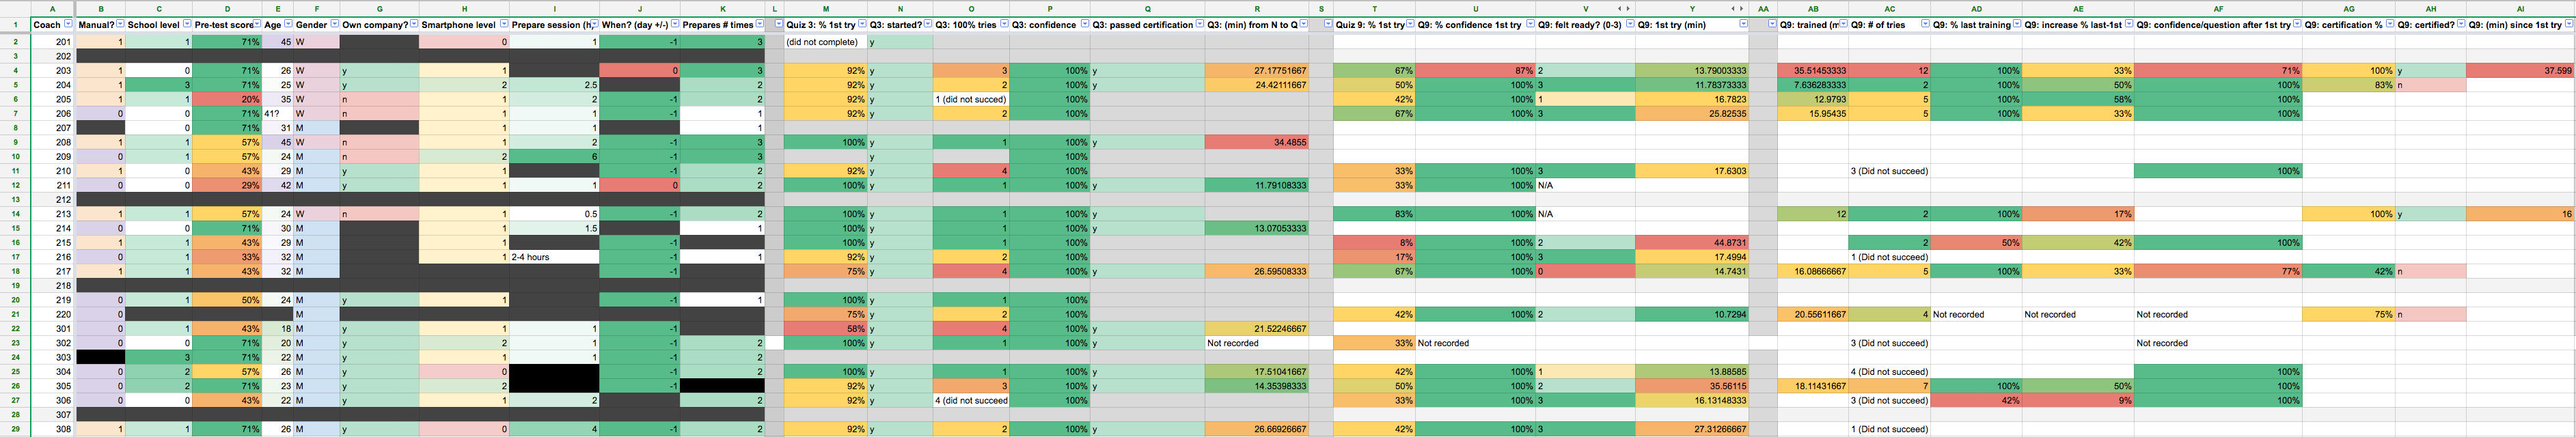
\includegraphics[width=.4\linewidth]{analysis/sheets/0Overview.png}
  \caption{A subfigure}
  \label{fig:sub1}
\end{subfigure}%
\begin{subfigure}{.5\textwidth}
  \centering
  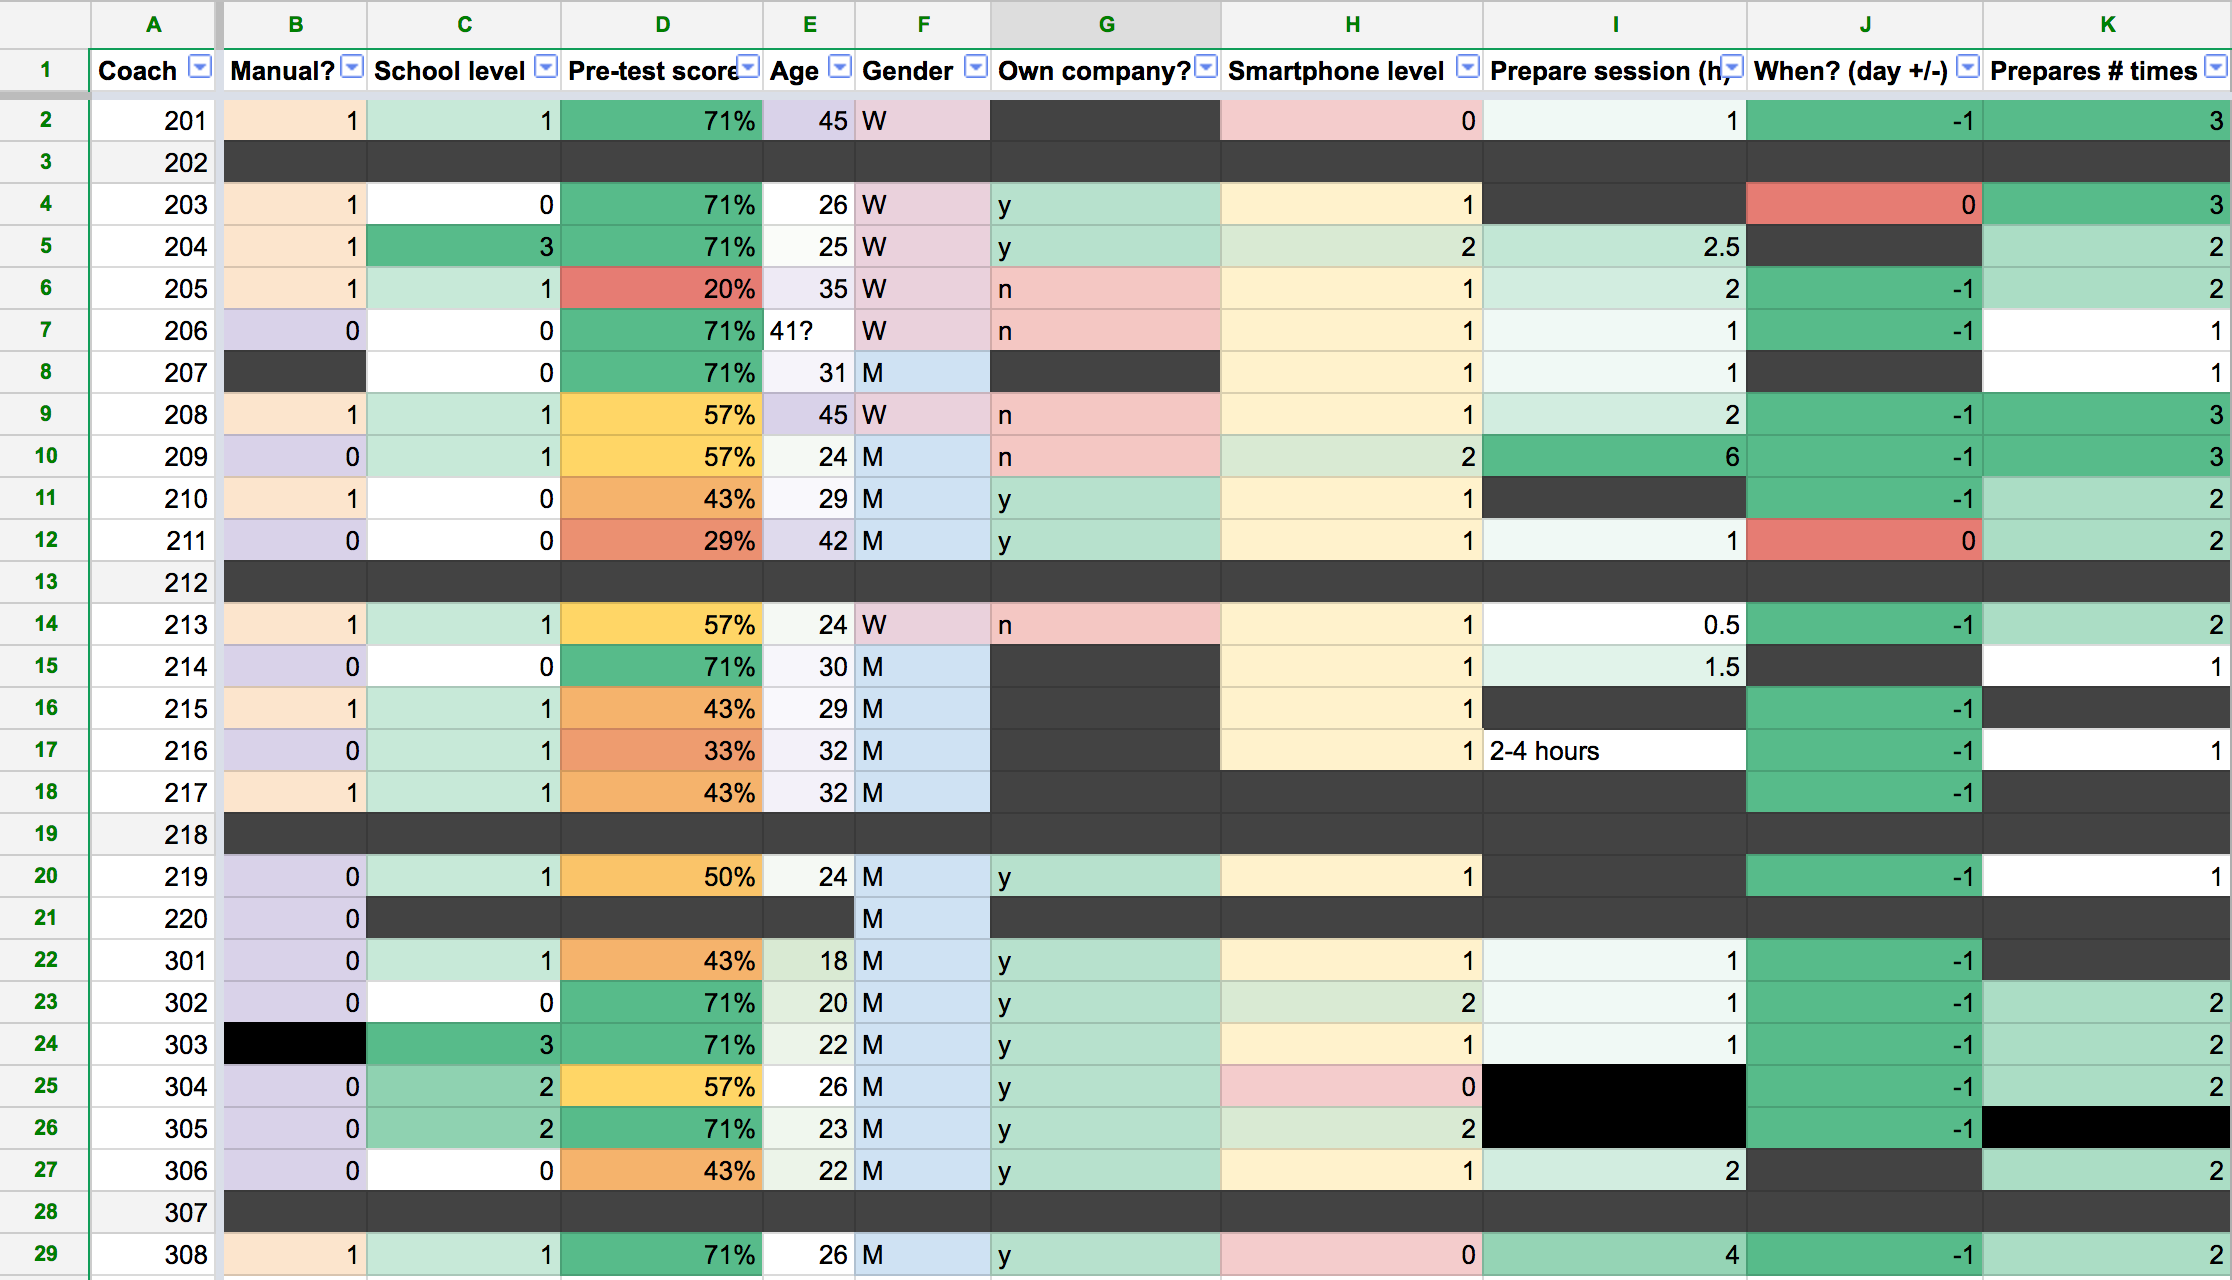
\includegraphics[width=.4\linewidth]{analysis/sheets/1Pre-data.png}
  \caption{A subfigure}
  \label{fig:sub2}
\end{subfigure}
\caption{A figure with two subfigures}
\label{fig:test}
\end{figure}


\begin{figure}[h]
    \centering
    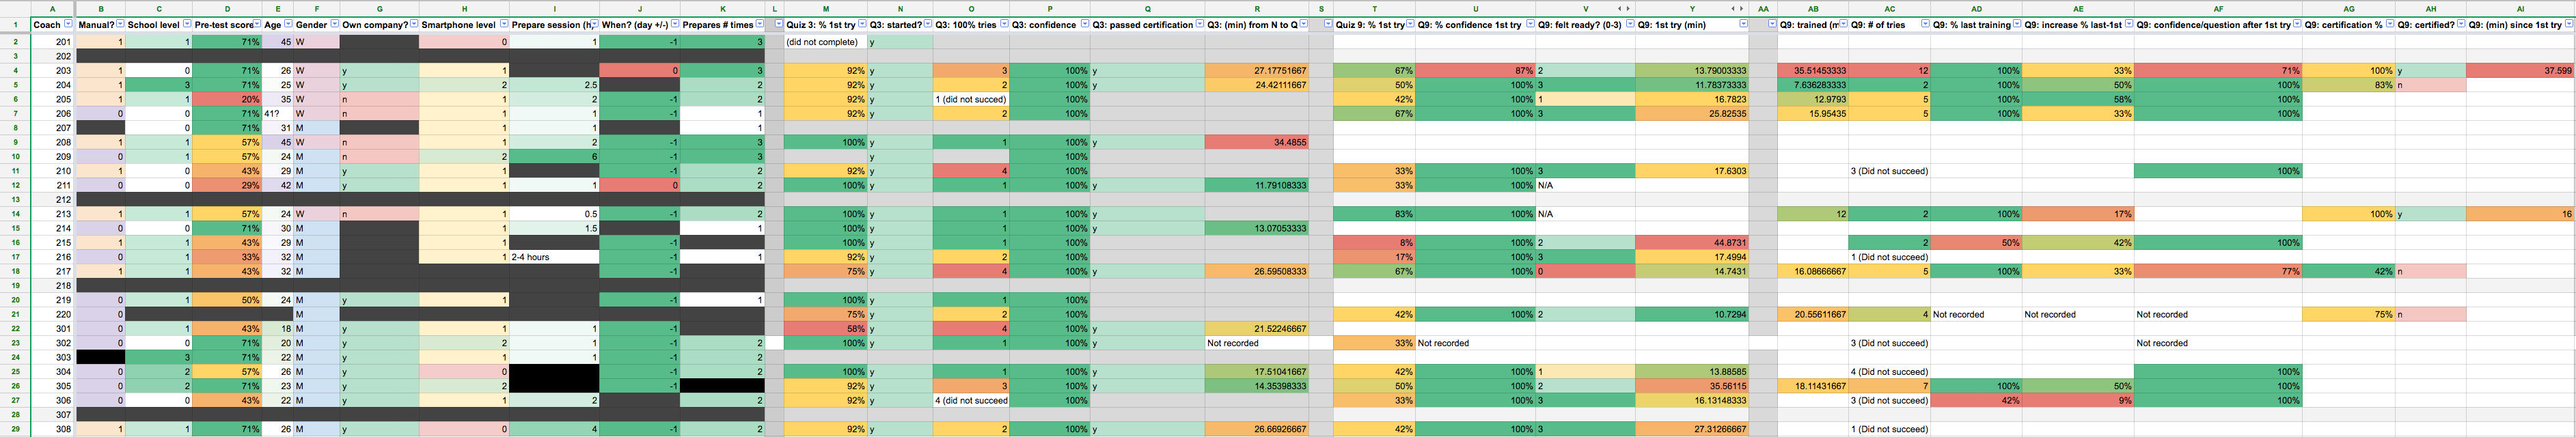
\includegraphics[width=1.0\textwidth]{analysis/sheets/0Overview.png}
    \caption{Overview}
    \label{fig:0}
\end{figure}

\begin{figure}[h]
    \centering
    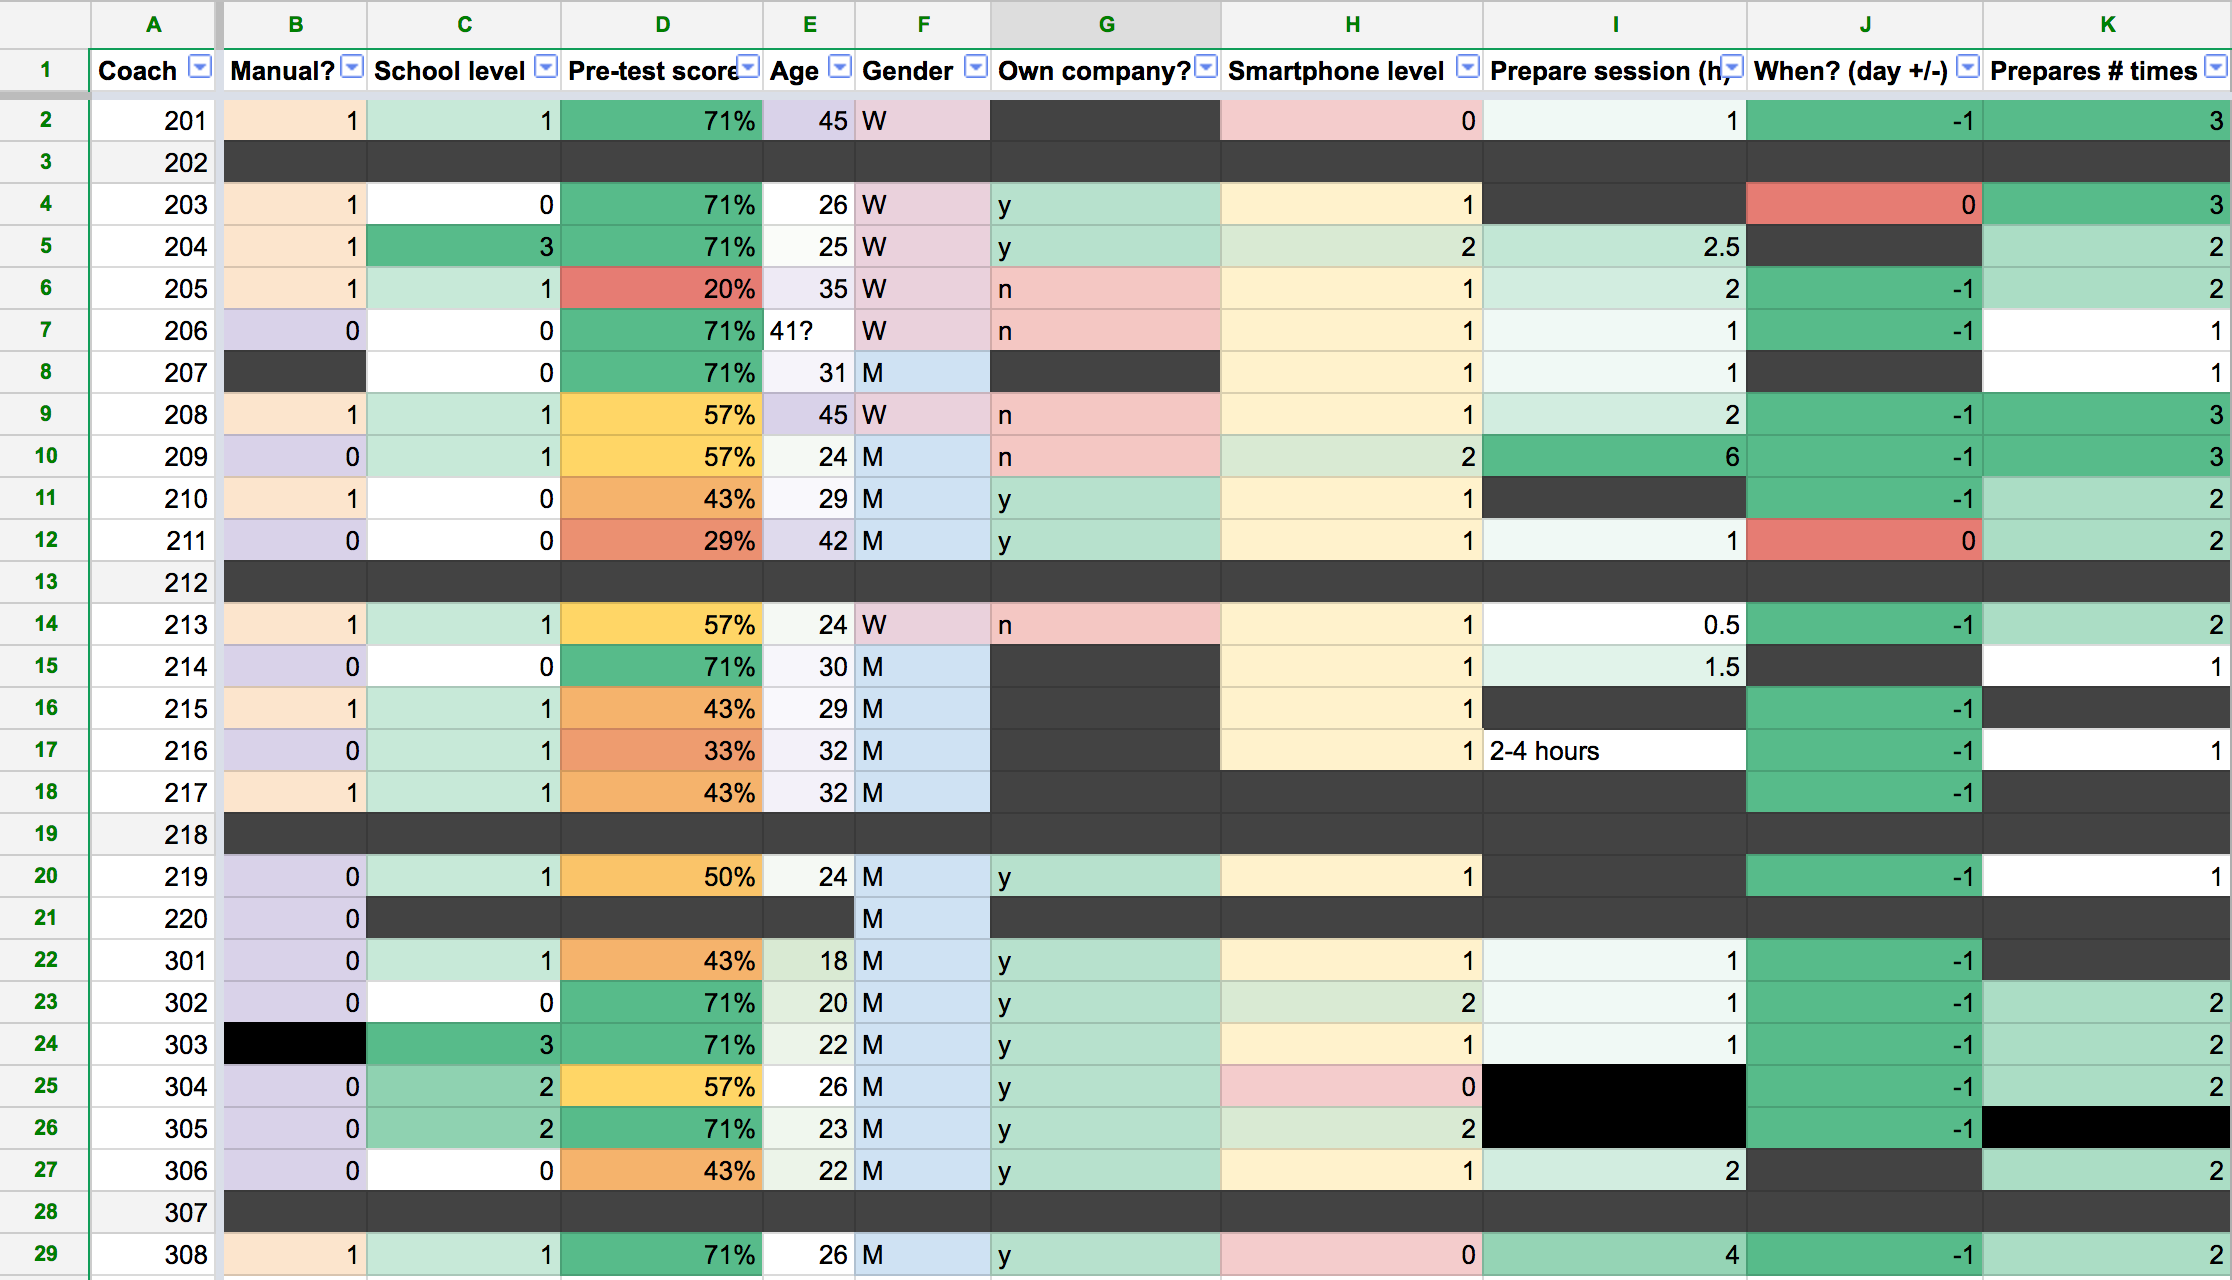
\includegraphics[width=1.0\textwidth]{analysis/sheets/1Pre-data.png}
    \caption{Pre-test data}
    \label{fig:1}
\end{figure}

\begin{figure}[h]
    \centering
    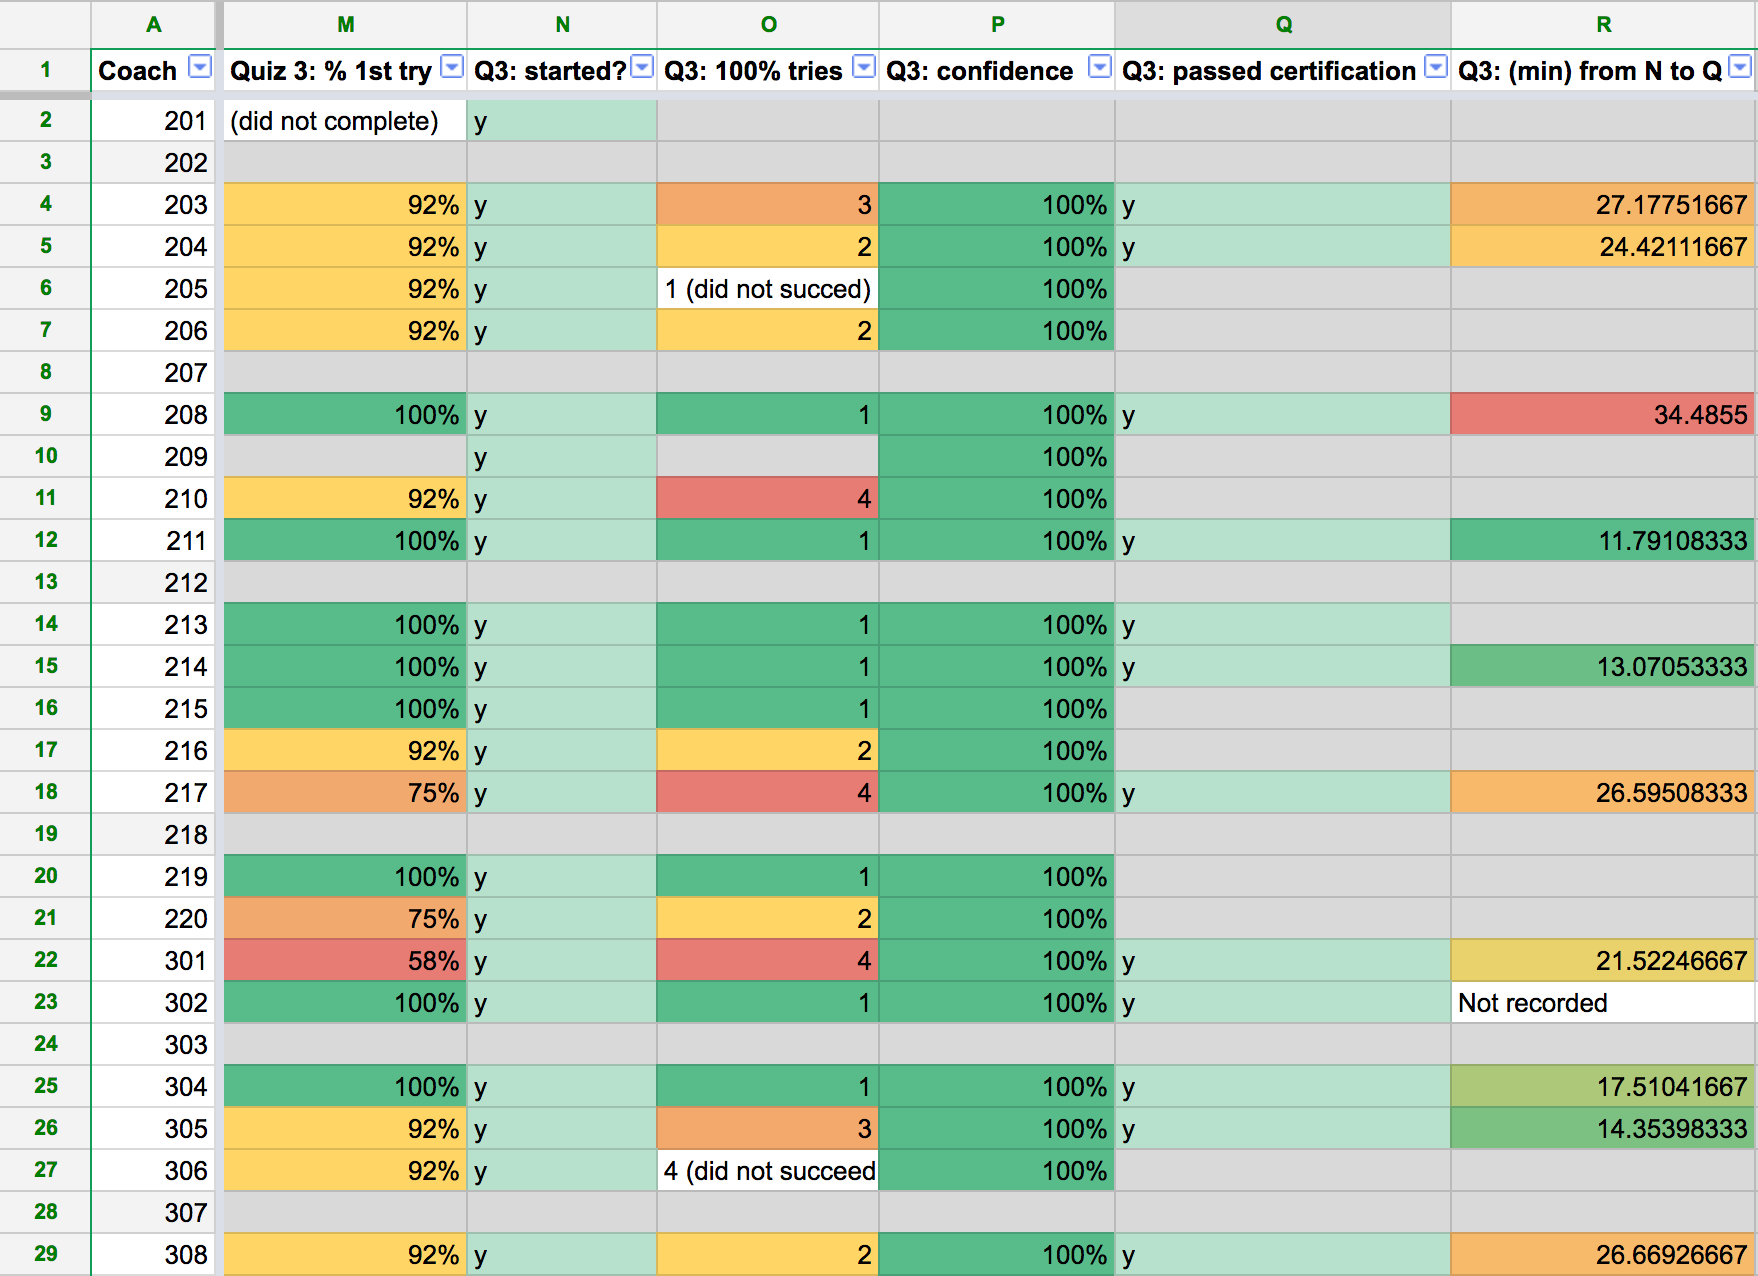
\includegraphics[width=1.0\textwidth]{analysis/sheets/2Quiz3.png}
    \caption{Quiz 3 answers}
    \label{fig:2}
\end{figure}

\begin{figure}[h]
    \centering
    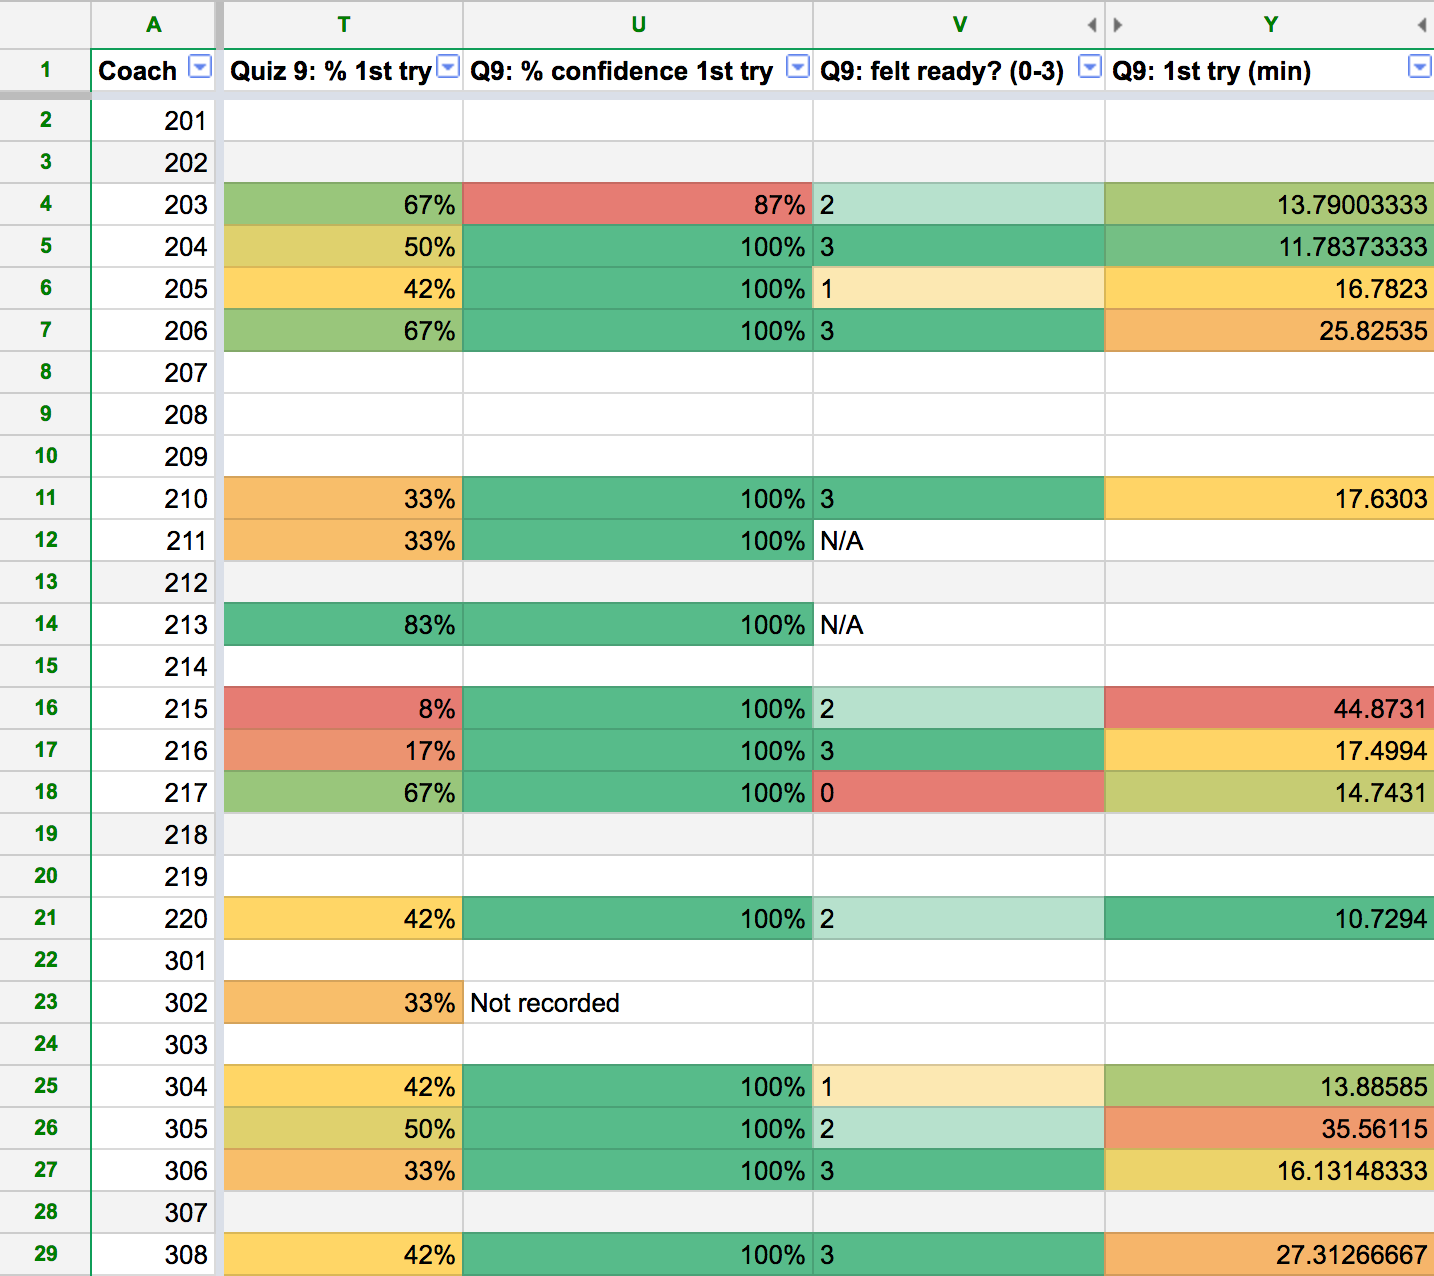
\includegraphics[width=1.0\textwidth]{analysis/sheets/3Quiz9A.png}
    \caption{Quiz 9 try 1 answers (correctness and recorded confidence ("Are you sure?": "Yes/%No") on coach guide quiz 9 "Are you ready?", together with answering "How comfortable and %ready do you feel right now to carry out session 9? (There is no right answer, just be %honest with yourself!", alternative 1-4 ("Not ready at all", "Somehow ready", "Ready" or "Very ready and comfortable"). Finally in column Y, the time it took for the coach to complete quiz try 1 is given.}
    \label{fig:3}
\end{figure}

\begin{figure}[h]
    \centering
    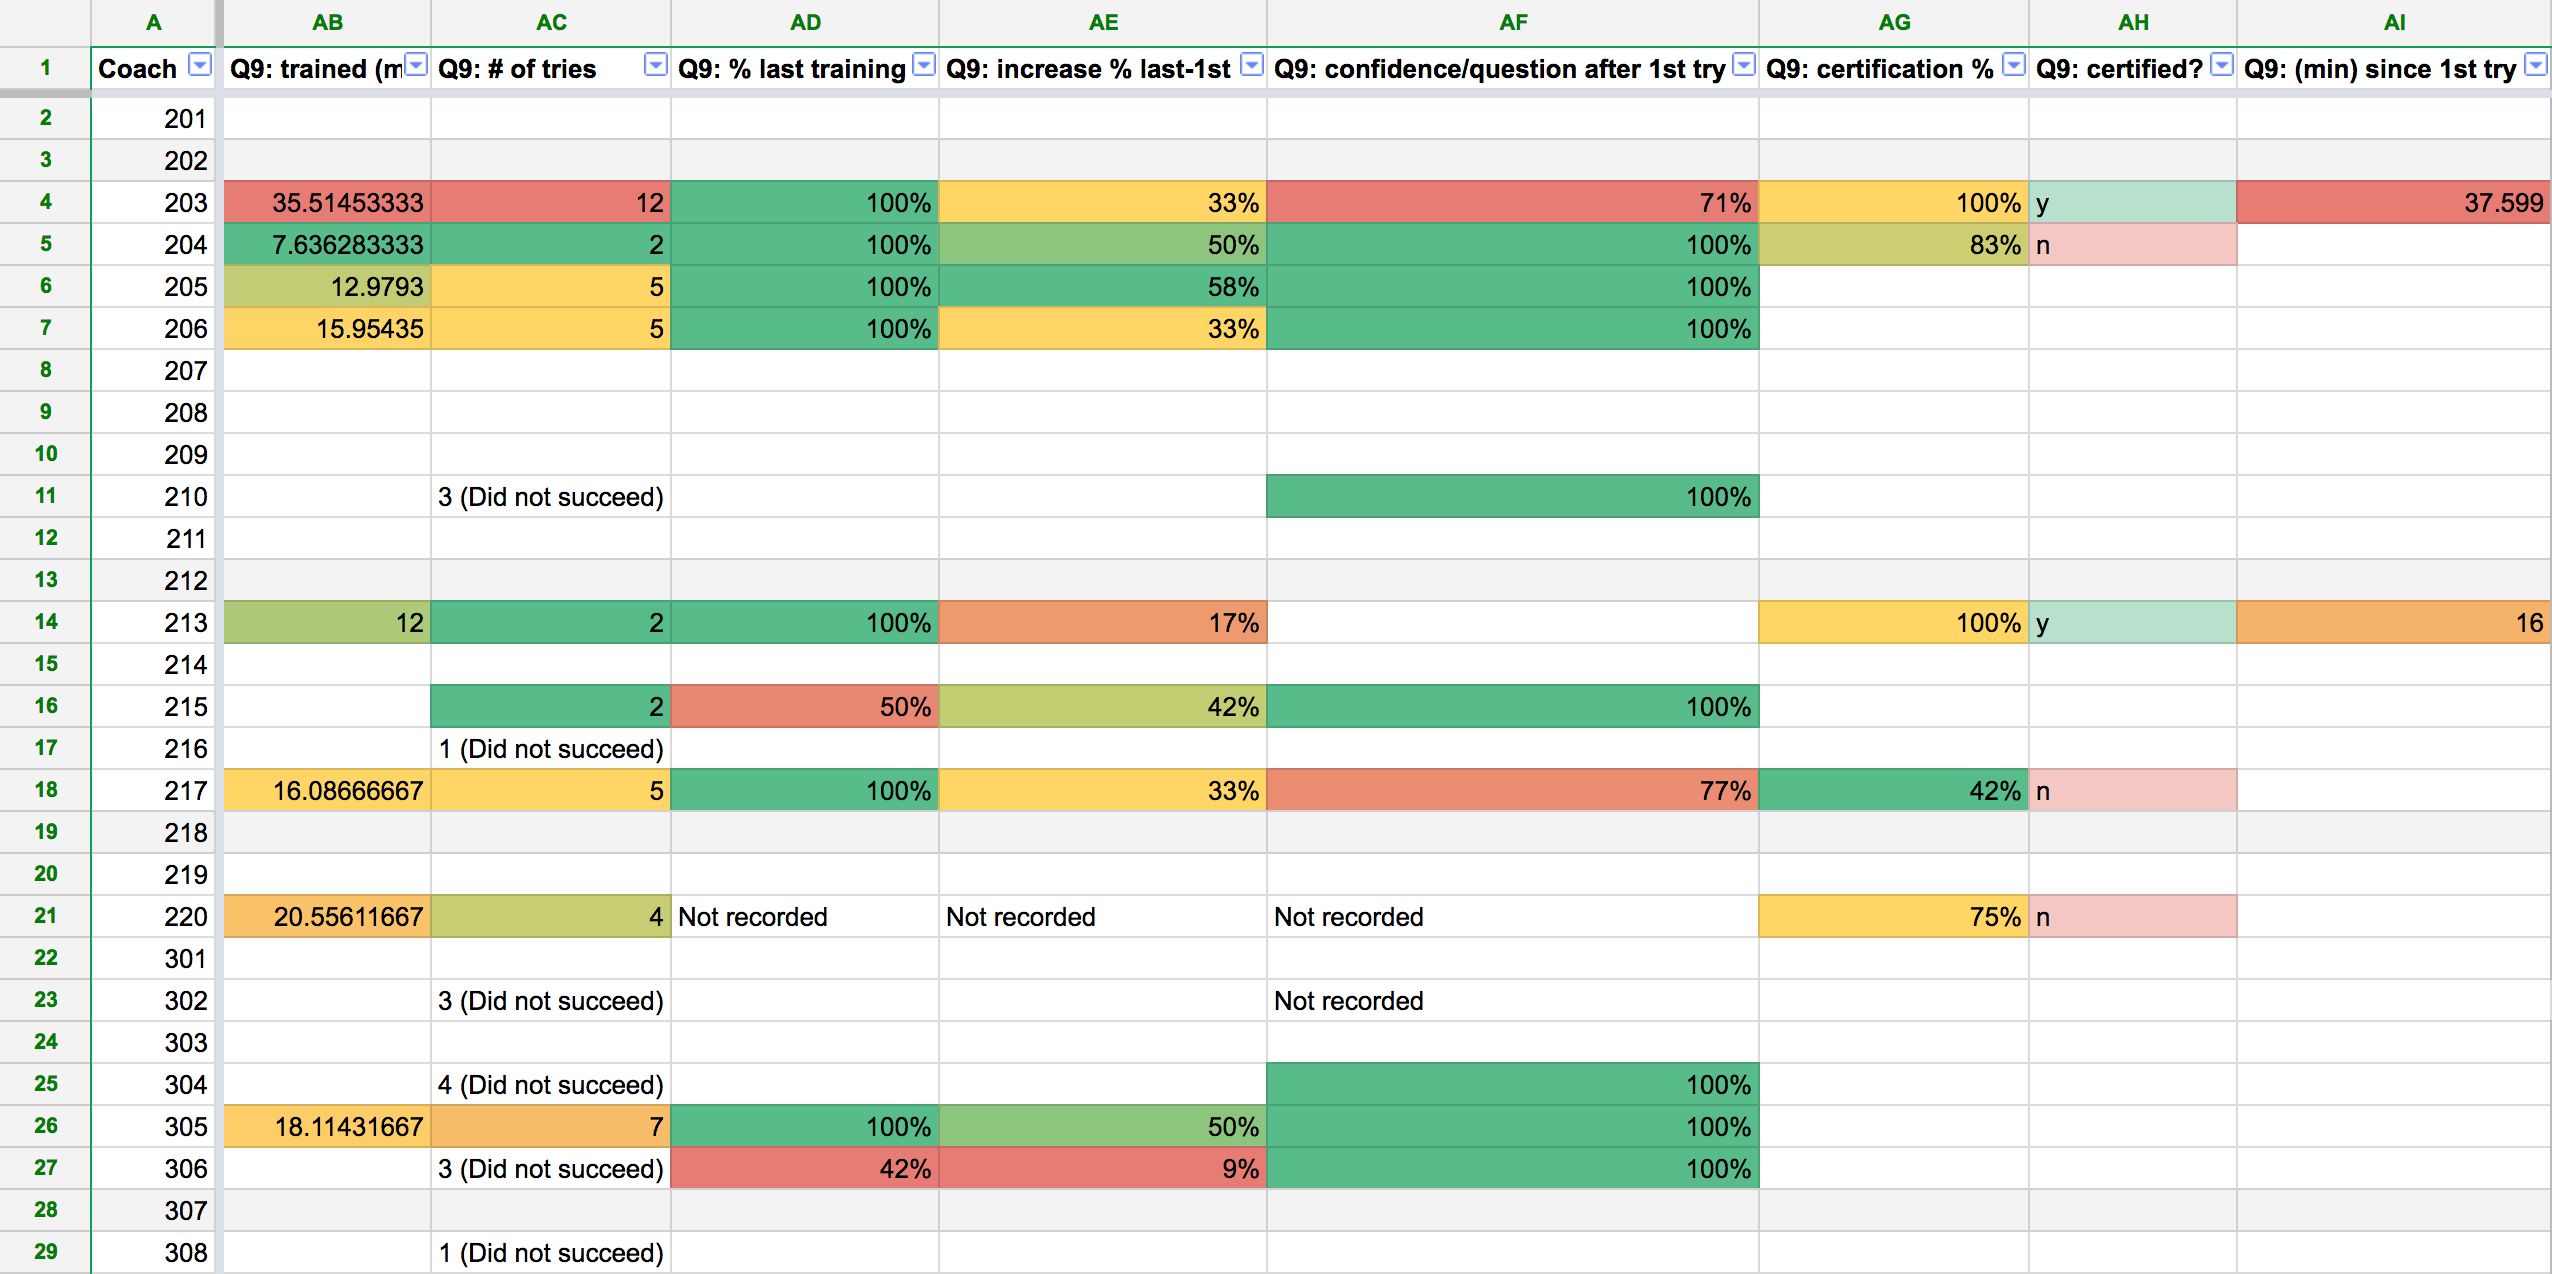
\includegraphics[width=1.0\textwidth]{analysis/sheets/3Quiz9B.png}
    \caption{Quiz results on the training and certification of coach guide quiz 9 "Are you ready?". Column AB: how many minutes they spent in training. AC: how many times they pressed "Try again", retaking the wrong answers. AD: their score on the last training quiz they took. AE: the increase from their first training to their last. AF: recorded "Are you sure?": "Yes/No" after taking the quiz try 1. Finally, for the coaches that started the certification, their results are shown, together with the time the quiz took for those that got 100\% correct on the first try.}
    \label{fig:4}
\end{figure}

\begin{figure}[h]
    \centering
    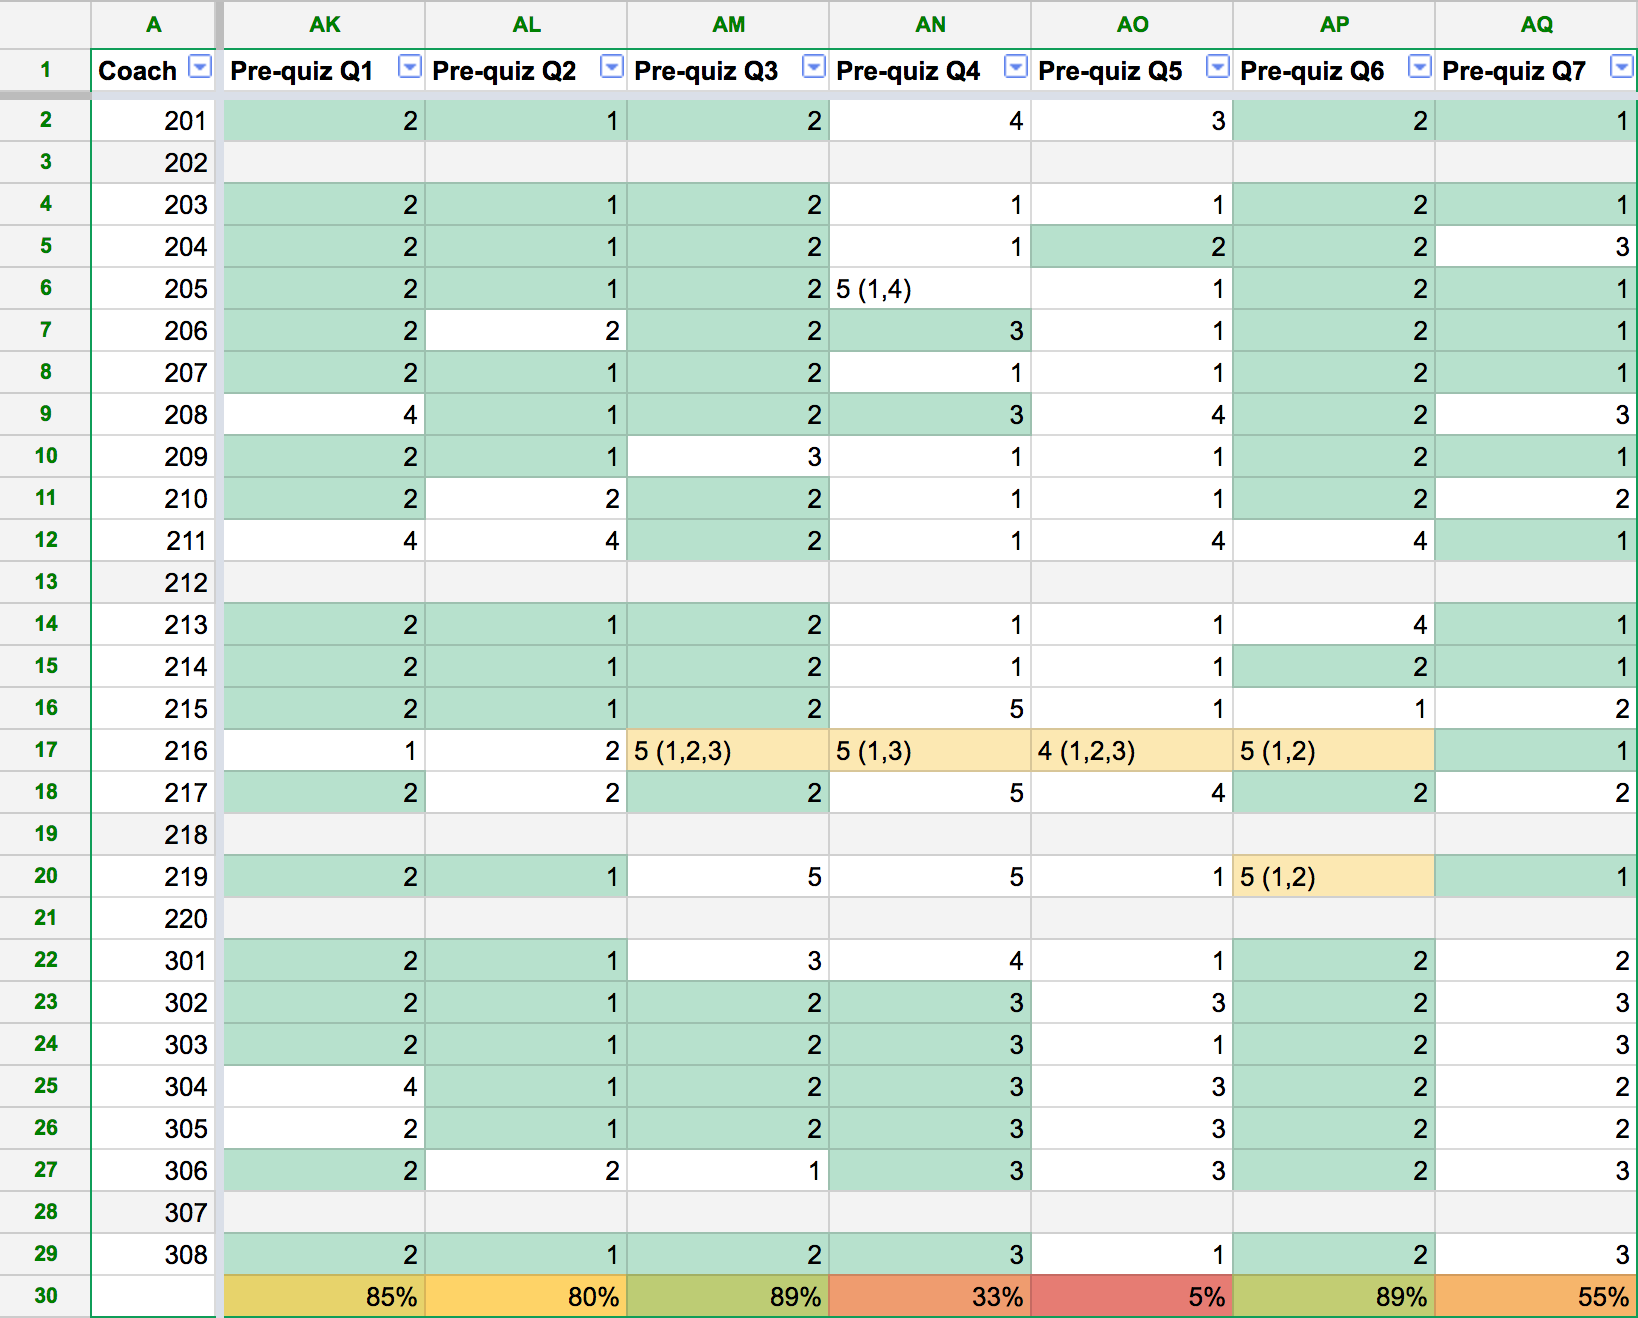
\includegraphics[width=1.0\textwidth]{analysis/sheets/4Pretest.png}
    \caption{Pre-quiz results per question and coach. The correct answers are given in green. The questions asked can be observed in Appendix \ref{cha:pre-test}}.}
    \label{fig:5}
\end{figure}
